\begin{tcolorbox}[
  title={\textbf{Box 3: How PCR primers work --- orientation on the template}},
  colback=teal!3!white, colframe=teal!50!black,
  fonttitle=\small\bfseries,
  left=6pt, right=6pt, top=4pt, bottom=4pt
]

\textbf{Key point.}
Forward and reverse primers are \emph{not} complementary to each other.
If they were, they would bind to \emph{each other} (primer dimers) instead of the DNA,
and PCR would fail.
Instead, each primer is complementary to \emph{one strand} of the template DNA at
\emph{opposite ends} of the target region, pointing toward each other.

\medskip
\begin{center}
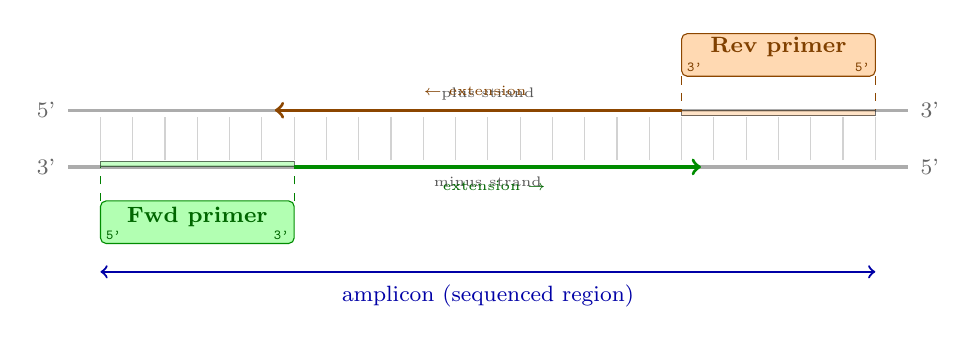
\begin{tikzpicture}[x=0.82cm, y=0.72cm, font=\small]

  % ── Genomic DNA double strand ──────────────────────────────────────
  % Plus strand (top): 5' → 3' left to right
  \draw[very thick, gray!65] (0,1) -- (13,1);
  \node[left,  font=\footnotesize, gray!80!black] at (-0.05,1) {5'};
  \node[right, font=\footnotesize, gray!80!black] at (13.05,1) {3'};
  \node[above, font=\tiny, gray!70!black] at (6.5,1) {plus strand};

  % Minus strand (bottom): 3' → 5' left to right  (5' → 3' right to left)
  \draw[very thick, gray!65] (0,0) -- (13,0);
  \node[left,  font=\footnotesize, gray!80!black] at (-0.05,0) {3'};
  \node[right, font=\footnotesize, gray!80!black] at (13.05,0) {5'};
  \node[below, font=\tiny, gray!70!black] at (6.5,0) {minus strand};

  % Base-pair ticks between strands
  \foreach \x in {0.5,1,...,12.5} {
    \draw[gray!35] (\x,0.12) -- (\x,0.88);
  }

  % ── Forward primer ─────────────────────────────────────────────────
  % Identical to the plus-strand sequence at the LEFT end of the target.
  % Anneals to the MINUS strand; extends rightward (→).
  \filldraw[fill=green!30, draw=green!55!black, rounded corners=2pt]
    (0.5,-1.35) rectangle (3.5,-0.6);
  \node[font=\footnotesize\bfseries, green!40!black] at (2,-0.88) {Fwd primer};
  % 5'→3' label on primer
  \node[font=\tiny, green!40!black] at (0.7,-1.2) {\texttt{5'}};
  \node[font=\tiny, green!40!black] at (3.3,-1.2) {\texttt{3'}};
  % dashed lines showing where it anneals on minus strand
  \draw[green!50!black, dashed, thin] (0.5,-0.6) -- (0.5, 0);
  \draw[green!50!black, dashed, thin] (3.5,-0.6) -- (3.5, 0);
  % highlight primer-binding region on minus strand
  \filldraw[fill=green!40, opacity=0.55] (0.5,0) rectangle (3.5,0.1);
  % extension arrow (new strand copies minus strand as template)
  \draw[->, very thick, green!55!black] (3.5,0) -- (9.8,0);
  \node[below, font=\tiny, green!40!black] at (6.6,-0.08) {extension $\rightarrow$};

  % ── Reverse primer ──────────────────────────────────────────────────
  % Identical to the minus-strand sequence at the RIGHT end of the target
  % (= reverse complement of the plus strand at that position).
  % Anneals to the PLUS strand; extends leftward (←).
  \filldraw[fill=orange!30, draw=orange!55!black, rounded corners=2pt]
    (9.5,1.6) rectangle (12.5,2.35);
  \node[font=\footnotesize\bfseries, orange!50!black] at (11,2.12) {Rev primer};
  % 5'→3' label (right to left because the primer runs 5'→3' rightward-to-leftward)
  \node[font=\tiny, orange!50!black] at (12.3,1.75) {\texttt{5'}};
  \node[font=\tiny, orange!50!black] at (9.7, 1.75) {\texttt{3'}};
  % dashed lines showing where it anneals on plus strand
  \draw[orange!55!black, dashed, thin] (9.5, 1.6) -- (9.5, 1);
  \draw[orange!55!black, dashed, thin] (12.5,1.6) -- (12.5,1);
  % highlight primer-binding region on plus strand
  \filldraw[fill=orange!40, opacity=0.55] (9.5,0.9) rectangle (12.5,1);
  % extension arrow (new strand copies plus strand as template)
  \draw[<-, very thick, orange!55!black] (3.2,1) -- (9.5,1);
  \node[above, font=\tiny, orange!50!black] at (6.3,1.08) {$\leftarrow$ extension};

  % ── Amplicon span ───────────────────────────────────────────────────
  \draw[<->, thick, blue!65!black] (0.5,-1.85) -- (12.5,-1.85);
  \node[below, blue!65!black, font=\footnotesize] at (6.5,-1.9) {amplicon (sequenced region)};

\end{tikzpicture}
\end{center}

\medskip
\textbf{What ``complementary'' actually means here.}
\begin{itemize}
  \item The \textcolor{green!50!black}{\textbf{forward primer}} is complementary to the
        \emph{minus strand} at the left end of the target. Its sequence is therefore
        identical to the plus strand at that position.
  \item The \textcolor{orange!60!black}{\textbf{reverse primer}} is complementary to the
        \emph{plus strand} at the right end of the target. Its sequence is the reverse
        complement of the plus strand at that position.
  \item The two primers are complementary to \emph{different strands at different loci}
        --- their sequences are unrelated to each other.
\end{itemize}

\medskip
\textbf{Why primer lengths differ within a pair.}
Primer length is tuned to achieve a target melting temperature ($T_m$).
Because $T_m$ depends on GC content as well as length, a GC-rich primer reaches the
required $T_m$ at a shorter length than an AT-rich primer.
Both primers in a pair need similar $T_m$ values (so both anneal at the same PCR
annealing temperature), but their lengths can therefore differ.
In this panel, lengths range from 21\,bp (\texttt{amplicon3\_rev}) to 30\,bp
(\texttt{amplicon1\_fwd/rev}, \texttt{amplicon3\_fwd}).

\end{tcolorbox}
